\documentclass[a4paper,12pt]{article}

\usepackage[margin=1in]{geometry}
\usepackage{tikz}
\usepackage{amssymb}
\usepackage{xcolor}
\usepackage{circuitikz}
\usepackage{graphicx}

\newcommand{\ra}{$\rightarrow$}
\newenvironment{6mini}{
  \begin{minipage}{6cm}
}{
  \end{minipage}
}

\title{\texttt{Multiplexers}\\\hrulefill}
\author{module 10}
\date{\small{10/30/2023}}

\begin{document}
    \maketitle

    \section{Multiplexers}
        A multiplexer is an electronic switch \ra switches multiple inputs to one output. It does this according to a \textbf{select line}:
        \begin{itemize}
            \item Determine what input is swicthed to the output
            \item Passes an input to output
            \item Max \# of inputs = , where n is \# of select lines
        \end{itemize}
        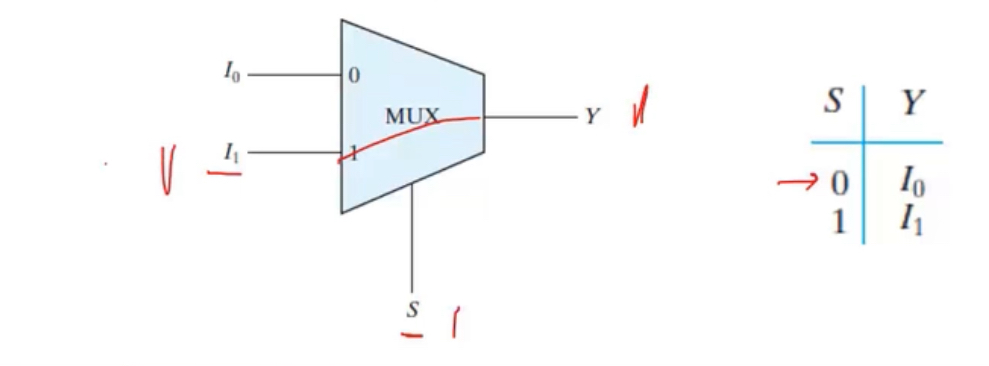
\includegraphics[width=10cm]{MultiplexerEx1.jpeg} \\
        \includegraphics*[width=10cm]{2nmultselct.jpeg}
        
        In the above image, $S_1$ is the MSB and $S_0$ is the LSB.
        \subsection{Inside of a Multiplexer}
        inside of a multiplexer uses the Laws of AND and OR. They are used to activate only one AND gate.
        \begin{itemize}
            \item A AND 1 is A
            \item A OR 0 is A
        \end{itemize}
        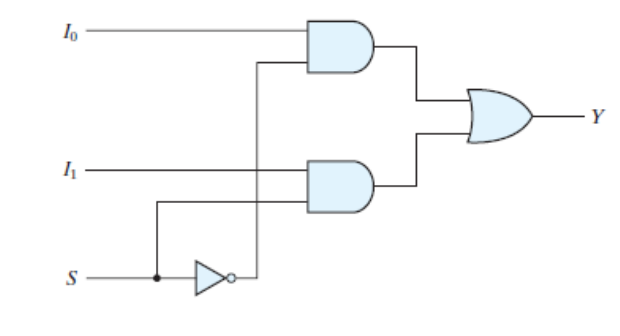
\includegraphics[width=8cm]{MultiSchem1.png}
        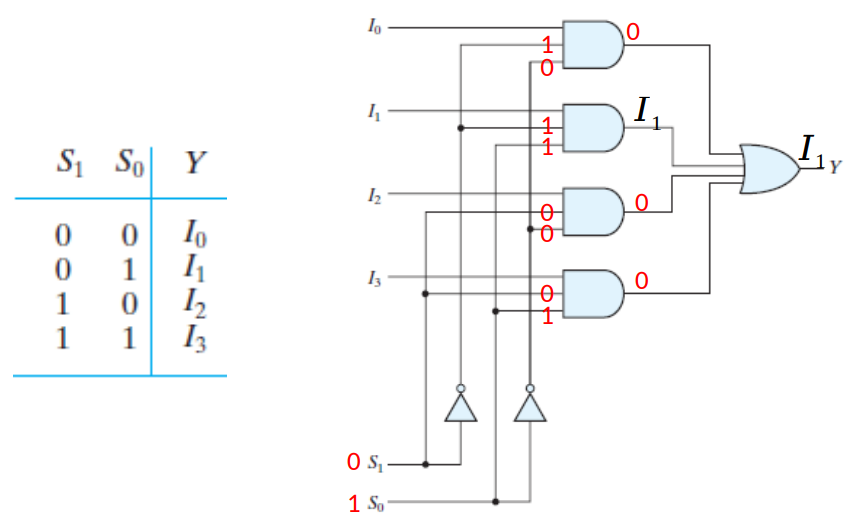
\includegraphics[width=8cm]{4inputmultischem.png}
        
        \section{Mutliple bit multiplexer}
            \textbf{A bus}
            \begin{itemize}
                \item Multiple bits passed through input or output
                \item number denotes how many bits are on said bus    
            \end{itemize}
            The figure below has a one bit enable and a 1 bit select line

            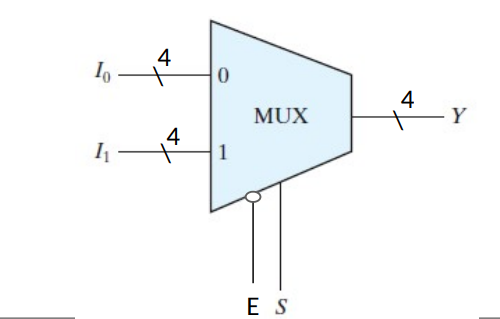
\includegraphics[width=6cm]{multbitmult.png}
            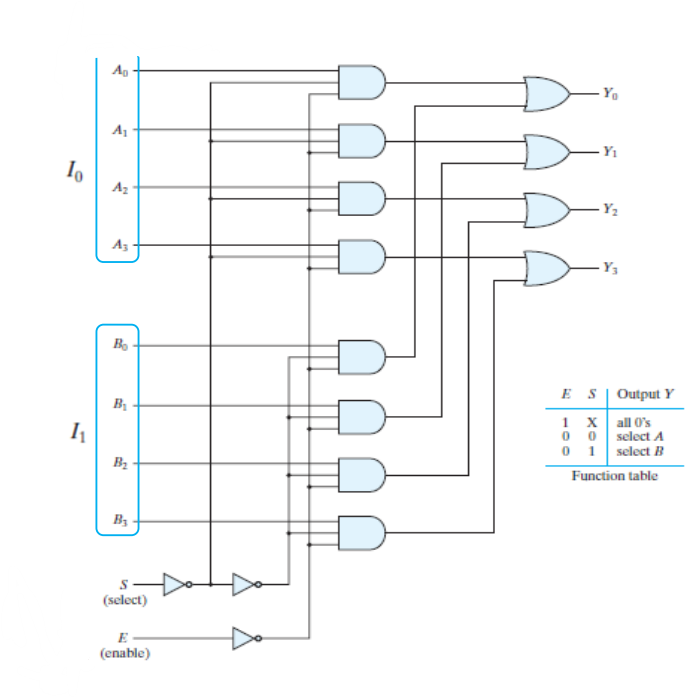
\includegraphics[width=10cm]{multbitmultschem.png}

            $I_0$ would be the LSB, while $I_1$ is the MSB.

            \subsection{Parallel multiplexer}
                achieving  abus input without so many logic gates everywhere \ra Placing the multiplxers in parellel will allow for bs inputs
                \begin{itemize}
                    \item \# multiplexers in parallel = number of bits on each bus inputsEach multiplexer will switch one digit of the multi-bit number
                    \item EX: one switches MSB while other swicthes LSB on 2 bit number
                \end{itemize}
                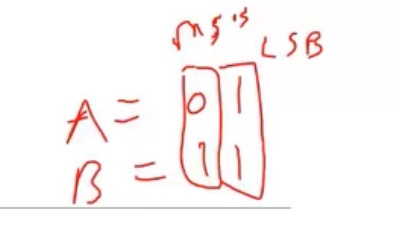
\includegraphics[width=4cm]{diagramforParallelmult.jpeg}
                \includegraphics*[width=12cm]{parallelMult.png}
                A0 would be the LSB of input A and A2 the MSB.

                \subsection{Cascading Multiplexers}
                    \begin{itemize}
                        \item Use the enable on multiplexer to create an additional select line
                        \item Connect remaining select lines together
                        \item OR outputs for each multiplexer
                    \end{itemize}
                    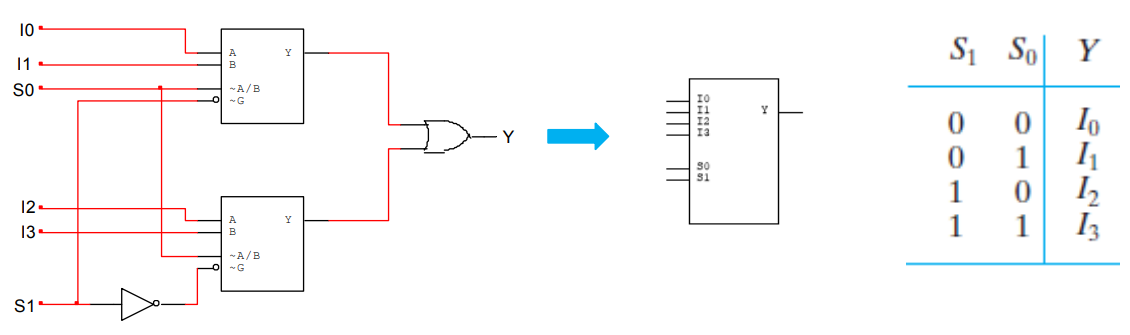
\includegraphics[width=16cm]{cascadeMult.png}\\
                    bottom multiplexer is the MSB multiplexer, top is the LSB in this example.
                    
                \section{Implementing Combinational Circuits}
                    Multiplexers can implement outputs of a truth table (\texttt{implementing minterms}).
                    \begin{itemize}
                        \item There will be one multiplexer per output.
                        \item number of select lines on multiplexers is \# inputs - 1
                        \item Remaining bits become the inpouts to the select lines
                        \item 3 inputs truth table uses 2 select lines, which is a 4 input multiplexer
                        \item Divide truth table rows by two, and compare how LSB changes to output. This becomes the input to the multiplexer
                    \end{itemize}
                    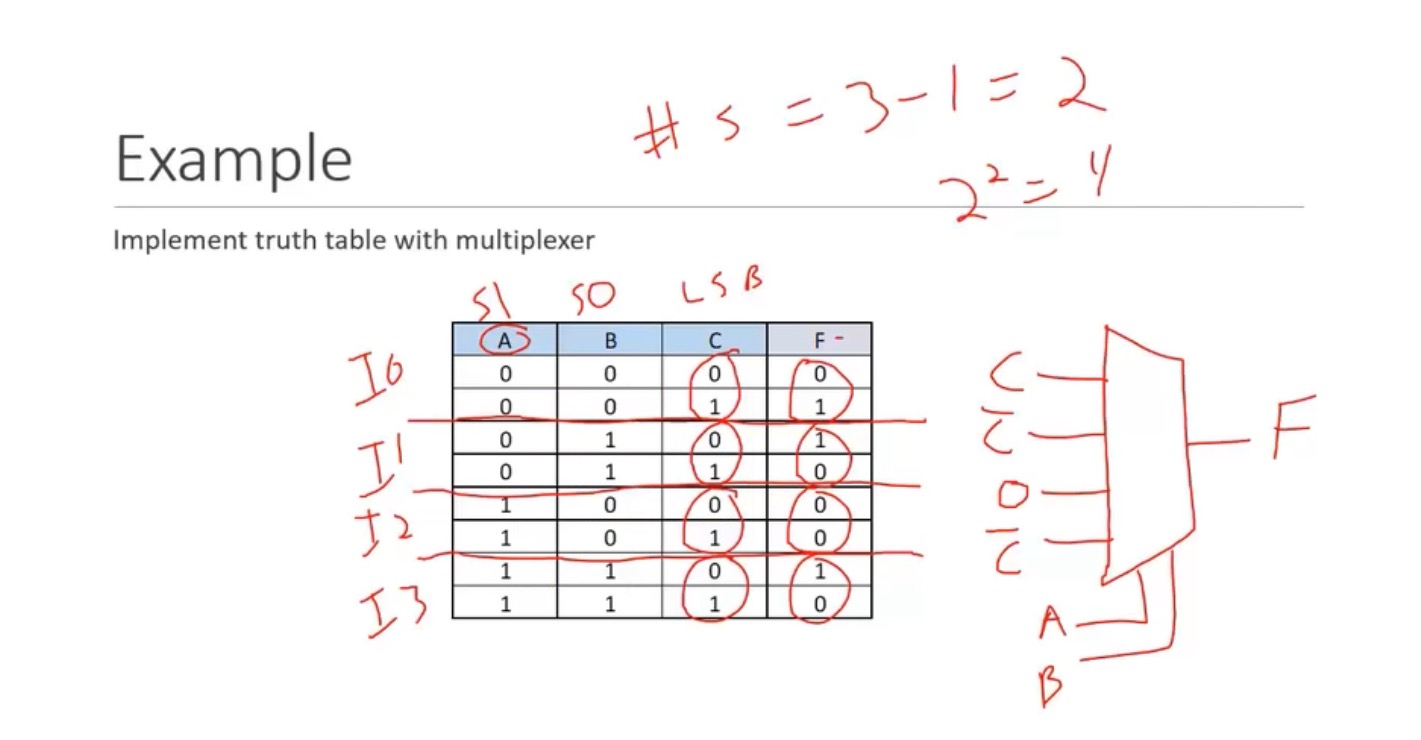
\includegraphics[width=14cm]{truthtomultEX1.jpeg}
\end{document}